% ==========================================================================================
% ==========================================================================================
% ==========================================================================================

\documentclass[10pt]{article}

% basic setup

\usepackage{microtype,graphicx,float,booktabs,verbatim,siunitx,titlesec,parskip,fullpage,nicefrac}
\usepackage[rsfs]{emf}  
\usepackage[version=4]{mhchem} 
\usepackage[bottom,hang]{footmisc}\setlength\footnotemargin{9pt}\interfootnotelinepenalty=10000\setlength{\skip\footins}{0.5cm}  

% tables and figures

\setlength\heavyrulewidth{0.2ex}\setlength\cmidrulewidth{0.1ex}\setlength\lightrulewidth{0.1ex}
\usepackage[font=normalsize,labelfont=bf]{caption}\captionsetup[table]{aboveskip=2pt}\captionsetup[figure]{skip=6pt}

% section headers

\titleformat{\section}{\large\bfseries}{\thetitle.}{.5em}{}
\titleformat{\subsection}{\bfseries}{\thesubsection.}{.5em}{}
\titleformat{\subsubsection}{\itshape}{\thesubsubsection.}{.5em}{}

% macros
    
\newcommand*\supr[1]{$^{#1}$}
\newcommand*\sub[1]{$_{#1}$}
\newcommand*\unit[1]{\textnormal{ #1}}
\newcommand*\rsq[1]{Correlation coefficient for line of best fit $R^2=#1$}

% labels

\def\tablab{Table}\def\tabslab{\tablab s}
\def\figlab{Figure}\def\figslab{\figlab s}
\def\equlab{Eq.}\def\equslab{Eqs.}
\newcommand*\eq[1]{\equlab~\ref{#1}}
\newcommand*\eqs[1]{\equslab~\ref{#1}}
\newcommand*\tbl[1]{\tablab~\ref{#1}}
\newcommand*\fig[1]{\figlab~\ref{#1}}
\newcommand*\figs[1]{\figslab~\ref{#1}}

% shortcuts

\def\deg{$^{\circ}$}
\def\tild{$\sim$}
\def\dg{$\Delta G$}
\def\electron{e$^-$}
\def\Ecell{$\emf_{\textnormal{cell}}$}
\def\Enotcell{$\emf^{\circ}_{\textnormal{cell}}$}
\def\Enot{$\emf^{\circ}$}
\def\not{^\circ}
\def\Ka{$K_{\textnormal{a}}$}
\def\Kb{$K_{\textnormal{b}}$}
\def\Kw{$K_{\textnormal{w}}$}
\def\Ksp{$K_{\textnormal{sp}}$}
\def\Keq{$K_{\textnormal{eq}}$}
\def\pKa{p$K_{\textnormal{a}}$}
\def\cmi{cm$^{-1}$}
\def\cd{$\cdot$}

% hyperref, load last

\usepackage{hyperref}\hypersetup{colorlinks = true}


% ==========================================================================================
% ==========================================================================================
% ==========================================================================================

\begin{document}

\title{Common Equations Used in Chemistry}
\author{John Terhorst, Ph.D.}

\maketitle
\tableofcontents

% ==========================================================================================
% ==========================================================================================
% ==========================================================================================

\newpage\section{Basic Conversions and Definitions}

Converting \deg F to \deg C:
\begin{equation*}
\textnormal{\deg C} = (\textnormal{\deg F}-32)\times \frac{5}{9}
\end{equation*}

Converting \deg C to \deg F:
\begin{equation*}
\textnormal{\deg F} = \left(\textnormal{\deg C}\times \frac{9}{5}\right) +32
\end{equation*}

Converting \deg C to K:
\begin{equation*}
K = \textnormal{\deg C}+273.15
\end{equation*}

% ==========================================================================================
% ==========================================================================================
% ==========================================================================================

\section{Solutions}

Density:
\begin{equation*}
d = \frac{m}{V}
\end{equation*}

Molarity:
\begin{equation*}
C = \frac{\textnormal{moles of solute}}{\textnormal{liters of solution}}
\end{equation*}

Molality:
\begin{equation*}
b = \frac{\textnormal{moles of solute}}{\textnormal{kg of solvent}}
\end{equation*}

Boiling point elevation\footnote{The van't Hoff factor, $i$, describes the number of particles formed upon solvation. For example, for solvation of sodium chloride, NaCl$(s)$ \ce{->} Na$^{+}(aq)$ + Cl$^{-}(aq)$, $i=2$. For a nonelectrolyte (like glucose or benzene), $i=1$. This factor can deviate from ideality for highly charged ions, where ion-pairing occurs (incomplete dissociation), as is seen with CaCl$_{2}$, where $i=2.6$ instead of 3.0 (CaCl$_{2}(s)$ \ce{->} Ca$^{2+}(aq)$ + 2Cl$^{-}(aq)$).}:
\begin{equation*} 
\Delta T_\textnormal{b} = iK_\textnormal{b}b
\end{equation*}

Freezing point depression:
\begin{equation*}
\Delta T_\textnormal{f} = iK_\textnormal{f}b
\end{equation*}

\begin{table}[H]
	\centering
	\caption{Boiling point elevation and freezing point depression constants for different solvents.}
		\begin{tabular}{cSSSS}
			\toprule
            Solvent & {Normal Boiling Point (\deg C)} & {$K_\textnormal{b}$ (\deg C/m)} & {Normal Freezing Point (\deg C)} & {$K_\textnormal{f}$ (\deg C/m)} \\ 
            \midrule
            Water & 100.0 & 0.512 & 0.0 & 1.86\\
            Acetic acid & 118.1 & 3.04 & 16.6 & 3.90\\
            Benzene & 80.1 & 2.53 & 5.5 & 5.12  \\
            Chloroform & 61.3 & 3.63 & -63.5 & 4.86\\
            Nitrobenzene & 210.9 & 5.24 & 5.67 & 8.1 \\
            \bottomrule
		\end{tabular}
\end{table}

Osmotic pressure:
\begin{equation*}
\pi=i\textnormal{M}RT
\end{equation*}

Dilution:
\begin{equation*}
C_1V_1=C_2V_2
\end{equation*}

% ==========================================================================================
% ==========================================================================================
% ==========================================================================================

\section{Gases}

% ==========================================================================================
% ==========================================================================================
% ==========================================================================================

Ideal Gas Law, $R=0.08206$ $\frac{\textnormal{L\cd atm}}{\textnormal{K\cd mol}}$
\begin{equation*}
PV=nRT
\end{equation*}

Boyle's Law ($n$, $T$ constant):
\begin{equation*}
P_1V_1=P_2V_2
\end{equation*}

Charles' Law ($n$, $P$ constant):
\begin{equation*}
\frac{V_1}{V_2} = \frac{T_1}{T_2} 
\end{equation*}

Avogadro's Law ($P$, $T$ constant):
\begin{equation*}
\frac{V_1}{V_2} = \frac{n_1}{n_2} 
\end{equation*}

Gay-Lussac's Law ($P$, $T$ constant):
\begin{equation*}
\frac{P_1}{P_2} = \frac{T_1}{T_2} 
\end{equation*}

Combined Gas Law ($n$ is constant):
\begin{equation*}
\frac{P_1V_1}{T_1} = \frac{P_2V_2}{T_2}
\end{equation*}

Relation of density to molar mass:
\begin{equation*}
M = \frac{dRT}{P}
\end{equation*}

Dalton's Law of Partial Pressures, where $\chi_i$ = mole fraction of species $i$ and $P_\textnormal{T}$ is total pressure:
\begin{equation*}
P_i=\chi_iP_\textnormal{T}
\end{equation*} 

Raoult's Law, where $P_i^\star$ is the vapor pressure of pure substance $i$:
\begin{equation*}
P_T^\star=\chi_\textnormal{A}P_\textnormal{A}^\star + \chi_\textnormal{B}P_\textnormal{Bb}^\star + \dots
\end{equation*}

Alternately,
\begin{equation*}
P_i=\chi_iP_i^\star
\end{equation*}

Root-mean-square (RMS) speed of a gas particle:
\begin{equation*}
\mu = \sqrt{\frac{3RT}{M}}
\end{equation*}

Rates of Effusion by Molar Mass
\begin{equation*}
\frac{\textnormal{rate}_1}{\textnormal{rate}_2} = \sqrt{\frac{M_2}{M_1}}
\end{equation*}

van der Waals equation for pressure of a non-ideal gas, where $a$ corrects for the attractive forces between gas particles, and $b$ corrects for the volume occupied by gas particles:
\begin{equation*}
\left(P+\frac{an^2}{V^2}\right)(V-nb)=nRT
\end{equation*}

% ==========================================================================================
% ==========================================================================================
% ==========================================================================================

\section{Thermodynamics}

% ==========================================================================================
% ==========================================================================================
% ==========================================================================================

\subsection{Heat Exchange}

Heat exchange, where $C_s$ is specific heat capacity:
\begin{equation*}
q=mC_s\Delta T
\end{equation*}

Calorimetry in an imperfect calorimeter:
\begin{equation*}
q_\textnormal{rxn}=mC_s\Delta T + C_\textnormal{cal}\Delta T
\end{equation*}

Heat exchange, where $C_V$ is molar heat capacity at constant volume:
\begin{equation*}
q= nC_V\Delta T
\end{equation*}

Heat exchange, where $C_P$ is molar heat capacity at constant pressure:
\begin{equation*}
q= nC_P\Delta T
\end{equation*}

% ==========================================================================================
% ==========================================================================================
% ==========================================================================================

\subsection{Conditions}

\subsubsection{Definitions}
\begin{itemize}
    \item Isothermal: $\Delta T = 0$, $\Delta E = 0$, $q = -w$
    \item Adiabatic: $q = 0$, $\Delta E = w$
    \item Isobaric: $\Delta P = 0$ (constant pressure)
\end{itemize}

\subsubsection{In General}
\begin{itemize}
    \item $q = nC\Delta T$
    \item $w = -P\Delta V$ where L$\cdot$atm = 101.325 J
    \item $\Delta E = q + w$
    \item $\Delta H = \Delta E + P\Delta V + V\Delta P$
    \item $C_\textnormal{P} = \frac{5}{2}R$ and $C_\textnormal{V} = \frac{3}{2}R$
\end{itemize}

\bigskip\begin{table}[H]
	\centering
	\caption{Summary of thermodynamic quantities under different conditions.}
		\begin{tabular}{lcccc}
			\toprule
            Quantity  & Constant $P$ & Constant $V$ & Adiabatic & Isothermal\\
            \midrule
            Heat, $q$    & $nC_\textnormal{P}\Delta T$ & $nC_\textnormal{V}\Delta T$ & 0 & $-w$ \\
            Work, $w$    & $-P\Delta V$ & 0 & $nC_V\Delta T$ & $-nRT\ln \left(\frac{V_\textnormal{f}}{V_\textnormal{i}}\right) = -nRT\ln \left(\frac{P_\textnormal{i}}{P_\textnormal{f}}\right)$ \\
            Energy, $\Delta E$ & $q+w$ & $q$ & $w$ & 0 \\
            Enthalpy, $\Delta H$ & $q$ & $\Delta E + V\Delta P$ & $V\Delta P$ & 0  \\
            Entropy, $\Delta S$ & $nC_\textnormal{P}\ln \left(\frac{T_\textnormal{f}}{T_\textnormal{i}}\right)$ &  $nC_\textnormal{V}\ln \left(\frac{T_\textnormal{f}}{T_\textnormal{i}}\right)$ & 0 & $nR\ln \left(\frac{V_\textnormal{f}}{V_\textnormal{i}}\right) = nR\ln \left(\frac{P_\textnormal{i}}{P_\textnormal{f}}\right)$ \\          
			\bottomrule
		\end{tabular}
	\label{cond}
\end{table}



% ==========================================================================================
% ==========================================================================================
% ==========================================================================================

\subsection{The Adiabatic Condition}

Given a rapid change in volume where $q=0$, both $P$ and $T$ change to accommodate the compression or expansion.
\begin{equation*}
\gamma = \frac{C_P}{C_V} = \frac{5}{3}
\end{equation*}

\begin{equation*}
(P_1)(V_1)^\gamma = (P_2)(V_2)^\gamma
\end{equation*}

\begin{equation*}
w = nC_V\Delta T
\end{equation*}

Temperature change in adiabatic compression or expansion:
\begin{equation*}
T_\textnormal{f} = T_\textnormal{i}\left(\frac{V_\textnormal{i}}{V_\textnormal{f}}\right)^{(R/C_V)}
\end{equation*}

% ==========================================================================================
% ==========================================================================================
% ==========================================================================================

% ==========================================================================================
% ==========================================================================================
% ==========================================================================================

\vspace*{0.5cm}
\subsection{Enthalpy}

Enthalpy is the energy required to create a system, plus the amount of energy required to make room for the system by displacing its environment by the system's volume at a given pressure.
\begin{equation*}
H = E + PV
\end{equation*}

Enthalpy change for a reaction:
\begin{equation*}
\Delta H = \Delta E + \Delta(PV) = \Delta E + P\Delta V + V\Delta P
\end{equation*}

Standard enthalpy of reaction, where $n$ and $m$ are coefficients in the balanced reaction equation:
\begin{equation*}
\Delta H\not_\textnormal{rxn} = \sum{n\Delta H\not_\textnormal{f}(\textnormal{products})}-\sum{m\Delta H\not_\textnormal{f}(\textnormal{reactants})} = \sum{D_\textnormal{broken}} - \sum{D_\textnormal{formed}} 
\end{equation*}

Clausius--Clapeyron equation:
\begin{equation*}
\ln P = \frac{-\Delta H_\textnormal{vap}}{RT}+C
\end{equation*}

Heat of vaporization based on the Clausius--Clapeyron equation:
\begin{equation*}
\ln \frac{P_1}{P_2} = \frac{\Delta H_\textnormal{vap}}{R}\left(\frac{1}{T_2} - \frac{1}{T_1}\right) = \frac{-\Delta H_\textnormal{vap}}{R}\left(\frac{1}{T_1} - \frac{1}{T_2}\right)
\end{equation*}

% ==========================================================================================
% ==========================================================================================
% ==========================================================================================

\newpage
\subsection{Entropy}

Second Law of Thermodynamics:
\begin{equation*}
\Delta S_\textnormal{universe} = \Delta S_\textnormal{system} + \Delta S_\textnormal{surroundings} > 0
\end{equation*}

Standard entropy of reaction, where $n$ and $m$ are coefficients in the balanced reaction equation:
\begin{equation*}
\Delta S\not_\textnormal{rxn} = \sum{n\Delta S\not(\textnormal{products})}-\sum{m\Delta S\not(\textnormal{reactants})}
\end{equation*}

Change in entropy with $\Delta H_{\textnormal{vap}}$ or $q$ where T is constant:
\begin{equation*}
\Delta S = \frac{\Delta H_{\textnormal{vap}}}{T} = \frac{q}{T}
\end{equation*}

Change in entropy with $\Delta V$ or $\Delta P$ where T is constant:
\begin{equation*}
\Delta S = nR\ln \left(\frac{V_\textnormal{f}}{V_\textnormal{i}}\right) = nR\ln \left(\frac{P_\textnormal{i}}{P_\textnormal{f}}\right)
\end{equation*}

Change in entropy for a thermodynamic process where T and/or P are varied:
\begin{equation*}
\Delta S = nC_V\ln\left(\frac{T_\textnormal{f}}{T_\textnormal{i}}\right) - nR\ln\left(\frac{P_\textnormal{f}}{P_\textnormal{i}}\right)
\end{equation*}

% ==========================================================================================
% ==========================================================================================
% ==========================================================================================

\subsection{Gibbs Free Energy}

Free energy change at constant temperature:
\begin{equation*}
\Delta G\not = \Delta H\not - T \Delta S\not
\end{equation*}

Or for an equilibrium reaction:
\begin{equation*}
\Delta G\not = -RT\ln K_{\textnormal{eq}}
\end{equation*}

Non-standard free energy:
\begin{equation*}
\Delta G = \Delta G\not + RT\ln Q
\end{equation*}

Standard free energy of reaction, where $n$ and $m$ are coefficients in the balanced reaction equation:
\begin{equation*}
\Delta G\not_\textnormal{rxn} = \sum{n\Delta G\not_\textnormal{f}(\textnormal{products})}-\sum{m\Delta G\not_\textnormal{f}(\textnormal{reactants})}
\end{equation*}

% ==========================================================================================
% ==========================================================================================
% ==========================================================================================



% ==========================================================================================
% ==========================================================================================
% ==========================================================================================

\newpage
\section{Electromagnetism}

% ==========================================================================================
% ==========================================================================================
% ==========================================================================================

Relationship of wavelength and frequency, where $c=\num{2.99e8}\unit{m/s}$:
\begin{equation*}
c = \lambda\nu
\end{equation*}

Energy of a photon, where Planck's constant $h=\num{6.626e-34}\unit{J\cd s}$:
\begin{equation*}
E = h\nu = \frac{hc}{\lambda}
\end{equation*}

Energy of an electron in the $n^{\textnormal{th}}$ shell in a hydrogen atom, where $R_\textnormal{H}=\num{2.18e-18}\unit{J}$:
\begin{equation*}
E_n=-Z^2R_\textnormal{H}\left(\frac{1}{n^2}\right)
\end{equation*}

Energy of a photon emitted as the electron undergoes a transition from the $n_\textnormal{i}$ shell to the $n_\textnormal{f}$ shell:
\begin{equation*}
\Delta E = Z^2R_\textnormal{H}\left(\frac{1}{n_\textnormal{f}^2}-\frac{1}{n_\textnormal{i}^2}\right)
\end{equation*}

Or, use $R_\textnormal{H} = 10973731.6$ m$^{-1}$:
\begin{equation*}
\frac{1}{\lambda} = Z^2R_\textnormal{H}\left(\frac{1}{n_\textnormal{f}^2}-\frac{1}{n_\textnormal{i}^2}\right)
\end{equation*}

de Broglie wavelength:
\begin{equation*}
\lambda=\frac{h}{mv}
\end{equation*}

Formal charge:
\begin{equation*}
q_\textnormal{F} = N_ie_\textnormal{V} - N_j\textnormal{B} - N_ke_\textnormal{NB} 
\end{equation*}

Dipole moment:
\begin{equation*}
\mu = Q\times r
\end{equation*}

Bragg equation:
\begin{equation*}
\lambda\nu = 2d \sin \theta
\end{equation*}

% ==========================================================================================
% ==========================================================================================
% ==========================================================================================
\newpage
\section{Quantum Mechanics}

Heisenberg Uncertainty Principle:
\begin{equation*}
\Delta x \Delta\rho \ge \frac{h}{4\pi}
\end{equation*}

The time-dependent Schr\"odinger equation:
\begin{equation*}
i\hbar\frac{\partial}{\partial t}|\Psi(t)\rangle = \hat{H}|\Psi(t)\rangle
\end{equation*}

The time-independent Schr\"odinger equation for a particle of mass $m$ moving in one direction with energy E where $\hbar=h/2\pi$ is:

\begin{equation*}
-\frac{\hbar^2}{2m}\frac{d^2\Psi(x)}{dx^2}+V(x)\Psi(x)=E\Psi(x)
\end{equation*}

Wavefunction for the $1s$ orbital:
\begin{equation*}
\psi_{1s} = \frac{1}{\sqrt{\pi}}e^{-r}
\end{equation*}

Wavefunction for the $2s$ orbital:
\begin{equation*}
\psi_{2s} = \frac{1}{2\sqrt{2\pi}}\left(1-\frac{r}{2}\right)e^{-r/2}
\end{equation*}

Wavefunction for the $2p_z$ orbital, where $a_0$ is the radius of the first Bohr orbit (\num{5.29e-11} m), $\sigma = Z(r/a_0)$ 
where $r$ is the distance (in m) from the nucleus and $Z$ is the nuclear charge, and $\theta$ is an angle:
\begin{equation*}
\psi_{2p_z} = \frac{1}{4\sqrt{2\pi}}\left(\frac{Z}{a_0}\right)^{3/2}\sigma e^{-\sigma/2}\cos\theta
\end{equation*}

Wavefunction for a particle in a 1-dimensional box of length L:
\begin{equation*}
\psi=\sqrt{\frac{2}{L}}\sin\left(\frac{n\pi}{L}\right)x
\end{equation*}

Energy for a particle in a 1-dimensional box of length L:
\begin{equation*}
E = \frac{n^2h^2}{8mL^2}
\end{equation*}

Potential energy between two charged bodies:
\begin{equation*}
V=k\frac{q_1q_2}{r}
\end{equation*}


% ==========================================================================================
% ==========================================================================================
% ==========================================================================================

\section{Stoichiometry}

Percent composition of an element in a compound, where $n$ = the number of moles of the element in one mole of the compound:
\begin{equation*}
\% = \left(\frac{n\times \textnormal{molar mass of element}}{\textnormal{molar mass of compound}}\right)\times 100\%
\end{equation*}

Percent yield:
\begin{equation*}
\textnormal{\% yield} = \left(\frac{\textnormal{actual yield}}{\textnormal{theoretical yield}}\right)\times 100\%
\end{equation*}

% ==========================================================================================
% ==========================================================================================
% ==========================================================================================

\newpage
\section{Electrochemistry}

% ==========================================================================================
% ==========================================================================================
% ==========================================================================================

Electrical force between two charged bodies:
\begin{equation*}
F_{e\ell}=k\frac{q_1q_2}{r_2}
\end{equation*}

Standard emf of an electrochemical cell:
\begin{equation*}
\textnormal{\Enotcell} = \textnormal{$\emf^{\hspace*{.5mm}\circ}_{\hspace*{-.3mm}\textnormal{ox}}$} - \textnormal{$\emf^{\hspace*{.5mm}\circ}_{\hspace*{.5mm}\textnormal{red}}$}  = \frac{RT}{nF} \ln K
\end{equation*}

Standard free energy of an electrochemical cell:
\begin{equation*}
\Delta G\not = -nF\textnormal{\Enotcell}
\end{equation*}

Nernst equation:
\begin{equation*}
\textnormal{\Ecell} = \textnormal{\Enotcell} - \frac{RT}{nF}\ln Q
\end{equation*}

Therefore:
Standard free energy of an electrochemical cell:
\begin{equation*}
\Delta G = -nF\textnormal{\Ecell}
\end{equation*}
% ==========================================================================================
% ==========================================================================================
% ==========================================================================================

\section{Reaction Kinetics}

\begin{table}[H]
    \centering
        \begin{tabular}{clll}
            \toprule
                \multicolumn{1}{c}{} & \multicolumn{3}{c}{Rate Laws}\\
                \cmidrule(l){2-4} 
                Order & Standard Form & Integrated Form & Line Form \\
                \midrule
                0 & $\textnormal{rate}=k$ & $\textnormal{[A]}_t-\textnormal{[A]}_0=-kt$ & $\textnormal{[A]}_t=-kt+\textnormal{[A]}_0$   \\[10pt]
                1 & $\textnormal{rate}=k\textnormal{[A]}$ & $\ln\frac{\textnormal{[A]}_t}{\textnormal{[A]}_0}=-kt$ & $\ln\textnormal{[A]}_t=-kt+\ln\textnormal{[A]}_0$  \\[10pt]
                2 & $\textnormal{rate}=k\textnormal{[A]}^2$ & $\frac{1}{\textnormal{[A]}_t}-\frac{1}{\textnormal{[A]}_0}=kt$ & $\frac{1}{\textnormal{[A]}_t}=kt+\frac{1}{\textnormal{[A]}_0}$  \\
            \bottomrule
        \end{tabular}
    \label{tabrate}
\end{table}

\begin{table}[H]
    \centering
        \begin{tabular}{cl}
            \toprule
                Order & Half-life\\
                \midrule
                0 & $t_{\nicefrac{1}{2}}=\frac{\textnormal{[A]}_0}{2k}$ \\[10pt]
                1 & $t_{\nicefrac{1}{2}}=\frac{\ln 2}{k}$  \\[10pt]
                2 & $t_{\nicefrac{1}{2}}=\frac{1}{k\textnormal{[A]}_0}$  \\
            \bottomrule
        \end{tabular}
    \label{tabhalf}
\end{table}

%The rate constant $k$ is a combination of many factors, mostly involving collision theory.\footnote{Collision theory is a theory that qualitatively explains how chemical reactions occur and why reaction rates differ for different reactions. Collision theory states that when suitable particles of the reactant collide with each other, only a certain percentage of the collisions cause any noticeable or significant chemical change; these successful changes are called ``successful collisions.'' A successful collision has enough energy, also known as activation energy ($E_\textnormal{a}$), at the moment of impact to break the preexisting bonds and form all new bonds. This results in the products of the reaction. Increasing the concentration of the reactant particles or raising the temperature, thus bringing about more collisions and therefore many more successful collisions, increases the rate of reaction.} It is defined by the 

Arrhenius equation:
\begin{equation*}
k = A \exp{\frac{-E_\textnormal{a}}{RT}}
\end{equation*}

Determining energy of activation:
\begin{equation*}
\ln k = \left(\frac{-E_\textnormal{a}}{R}\right)\left(\frac{1}{T}\right) + \ln A
\end{equation*}

Relationships of rate constants at two different temperatures:
\begin{equation*}
\ln \frac{k_1}{k_2} = \frac{E_\textnormal{a}}{R}\left(\frac{1}{T_2} - \frac{1}{T_1}\right) = \frac{-E_\textnormal{a}}{R}\left(\frac{1}{T_1}-\frac{1}{T_2}\right)
\end{equation*}

\subsection{Kinetics Data}

\begin{table}[htbp]
    \centering
    \caption{Kinetics Data --- 0th Order}
        \begin{tabular}{cccc}
            \toprule
                Time & Concentration & ln(Concentration) & 1/(Concentration) \\
                \midrule
                0     & 100   & 4.605 & 0.0100 \\
                1     & 90    & 4.499 & 0.0110 \\
                2     & 80    & 4.382 & 0.0125 \\
                3     & 70    & 4.248 & 0.0141 \\
                4     & 60    & 4.094 & 0.0166 \\
                5     & 50    & 3.912 & 0.0200 \\
                6     & 40    & 3.688 & 0.0250 \\
                7     & 30    & 3.401 & 0.0333 \\
            \bottomrule
        \end{tabular}
\end{table}
\vspace*{-.5cm}    
{\centering% GNUPLOT: LaTeX picture with Postscript
\begingroup
  \makeatletter
  \providecommand\color[2][]{%
    \GenericError{(gnuplot) \space\space\space\@spaces}{%
      Package color not loaded in conjunction with
      terminal option `colourtext'%
    }{See the gnuplot documentation for explanation.%
    }{Either use 'blacktext' in gnuplot or load the package
      color.sty in LaTeX.}%
    \renewcommand\color[2][]{}%
  }%
  \providecommand\includegraphics[2][]{%
    \GenericError{(gnuplot) \space\space\space\@spaces}{%
      Package graphicx or graphics not loaded%
    }{See the gnuplot documentation for explanation.%
    }{The gnuplot epslatex terminal needs graphicx.sty or graphics.sty.}%
    \renewcommand\includegraphics[2][]{}%
  }%
  \providecommand\rotatebox[2]{#2}%
  \@ifundefined{ifGPcolor}{%
    \newif\ifGPcolor
    \GPcolortrue
  }{}%
  \@ifundefined{ifGPblacktext}{%
    \newif\ifGPblacktext
    \GPblacktextfalse
  }{}%
  % define a \g@addto@macro without @ in the name:
  \let\gplgaddtomacro\g@addto@macro
  % define empty templates for all commands taking text:
  \gdef\gplbacktext{}%
  \gdef\gplfronttext{}%
  \makeatother
  \ifGPblacktext
    % no textcolor at all
    \def\colorrgb#1{}%
    \def\colorgray#1{}%
  \else
    % gray or color?
    \ifGPcolor
      \def\colorrgb#1{\color[rgb]{#1}}%
      \def\colorgray#1{\color[gray]{#1}}%
      \expandafter\def\csname LTw\endcsname{\color{white}}%
      \expandafter\def\csname LTb\endcsname{\color{black}}%
      \expandafter\def\csname LTa\endcsname{\color{black}}%
      \expandafter\def\csname LT0\endcsname{\color[rgb]{1,0,0}}%
      \expandafter\def\csname LT1\endcsname{\color[rgb]{0,1,0}}%
      \expandafter\def\csname LT2\endcsname{\color[rgb]{0,0,1}}%
      \expandafter\def\csname LT3\endcsname{\color[rgb]{1,0,1}}%
      \expandafter\def\csname LT4\endcsname{\color[rgb]{0,1,1}}%
      \expandafter\def\csname LT5\endcsname{\color[rgb]{1,1,0}}%
      \expandafter\def\csname LT6\endcsname{\color[rgb]{0,0,0}}%
      \expandafter\def\csname LT7\endcsname{\color[rgb]{1,0.3,0}}%
      \expandafter\def\csname LT8\endcsname{\color[rgb]{0.5,0.5,0.5}}%
    \else
      % gray
      \def\colorrgb#1{\color{black}}%
      \def\colorgray#1{\color[gray]{#1}}%
      \expandafter\def\csname LTw\endcsname{\color{white}}%
      \expandafter\def\csname LTb\endcsname{\color{black}}%
      \expandafter\def\csname LTa\endcsname{\color{black}}%
      \expandafter\def\csname LT0\endcsname{\color{black}}%
      \expandafter\def\csname LT1\endcsname{\color{black}}%
      \expandafter\def\csname LT2\endcsname{\color{black}}%
      \expandafter\def\csname LT3\endcsname{\color{black}}%
      \expandafter\def\csname LT4\endcsname{\color{black}}%
      \expandafter\def\csname LT5\endcsname{\color{black}}%
      \expandafter\def\csname LT6\endcsname{\color{black}}%
      \expandafter\def\csname LT7\endcsname{\color{black}}%
      \expandafter\def\csname LT8\endcsname{\color{black}}%
    \fi
  \fi
    \setlength{\unitlength}{0.0500bp}%
    \ifx\gptboxheight\undefined%
      \newlength{\gptboxheight}%
      \newlength{\gptboxwidth}%
      \newsavebox{\gptboxtext}%
    \fi%
    \setlength{\fboxrule}{0.5pt}%
    \setlength{\fboxsep}{1pt}%
\begin{picture}(4680.00,3276.00)%
    \gplgaddtomacro\gplbacktext{%
      \csname LTb\endcsname%%
      \put(1615,880){\makebox(0,0)[r]{\strut{}$30$}}%
      \csname LTb\endcsname%%
      \put(1615,1128){\makebox(0,0)[r]{\strut{}$40$}}%
      \csname LTb\endcsname%%
      \put(1615,1376){\makebox(0,0)[r]{\strut{}$50$}}%
      \csname LTb\endcsname%%
      \put(1615,1624){\makebox(0,0)[r]{\strut{}$60$}}%
      \csname LTb\endcsname%%
      \put(1615,1871){\makebox(0,0)[r]{\strut{}$70$}}%
      \csname LTb\endcsname%%
      \put(1615,2119){\makebox(0,0)[r]{\strut{}$80$}}%
      \csname LTb\endcsname%%
      \put(1615,2367){\makebox(0,0)[r]{\strut{}$90$}}%
      \csname LTb\endcsname%%
      \put(1615,2615){\makebox(0,0)[r]{\strut{}$100$}}%
      \csname LTb\endcsname%%
      \put(1747,660){\makebox(0,0){\strut{}$0$}}%
      \csname LTb\endcsname%%
      \put(1995,660){\makebox(0,0){\strut{}$1$}}%
      \csname LTb\endcsname%%
      \put(2243,660){\makebox(0,0){\strut{}$2$}}%
      \csname LTb\endcsname%%
      \put(2491,660){\makebox(0,0){\strut{}$3$}}%
      \csname LTb\endcsname%%
      \put(2738,660){\makebox(0,0){\strut{}$4$}}%
      \csname LTb\endcsname%%
      \put(2986,660){\makebox(0,0){\strut{}$5$}}%
      \csname LTb\endcsname%%
      \put(3234,660){\makebox(0,0){\strut{}$6$}}%
      \csname LTb\endcsname%%
      \put(3482,660){\makebox(0,0){\strut{}$7$}}%
    }%
    \gplgaddtomacro\gplfronttext{%
      \csname LTb\endcsname%%
      \put(999,1747){\rotatebox{-270}{\makebox(0,0){\strut{}Concentration}}}%
      \put(2614,330){\makebox(0,0){\strut{}Time (s)}}%
      \put(2614,2945){\makebox(0,0){\strut{}0th Order Plot, $R^2$ = 1}}%
      \csname LTb\endcsname%%
      \put(2495,2442){\makebox(0,0)[r]{\strut{}fit}}%
    }%
    \gplbacktext
    \put(0,0){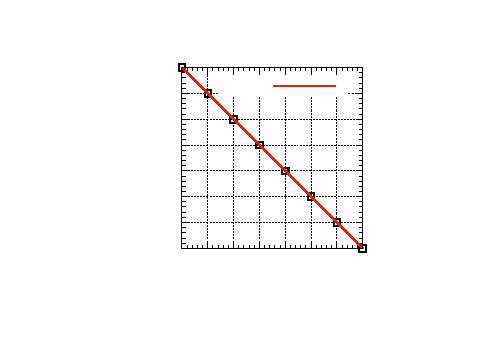
\includegraphics{kinetics/0/0a/mygraph}}%
    \gplfronttext
  \end{picture}%
\endgroup
\\[-3.5ex]
% GNUPLOT: LaTeX picture with Postscript
\begingroup
  \makeatletter
  \providecommand\color[2][]{%
    \GenericError{(gnuplot) \space\space\space\@spaces}{%
      Package color not loaded in conjunction with
      terminal option `colourtext'%
    }{See the gnuplot documentation for explanation.%
    }{Either use 'blacktext' in gnuplot or load the package
      color.sty in LaTeX.}%
    \renewcommand\color[2][]{}%
  }%
  \providecommand\includegraphics[2][]{%
    \GenericError{(gnuplot) \space\space\space\@spaces}{%
      Package graphicx or graphics not loaded%
    }{See the gnuplot documentation for explanation.%
    }{The gnuplot epslatex terminal needs graphicx.sty or graphics.sty.}%
    \renewcommand\includegraphics[2][]{}%
  }%
  \providecommand\rotatebox[2]{#2}%
  \@ifundefined{ifGPcolor}{%
    \newif\ifGPcolor
    \GPcolortrue
  }{}%
  \@ifundefined{ifGPblacktext}{%
    \newif\ifGPblacktext
    \GPblacktextfalse
  }{}%
  % define a \g@addto@macro without @ in the name:
  \let\gplgaddtomacro\g@addto@macro
  % define empty templates for all commands taking text:
  \gdef\gplbacktext{}%
  \gdef\gplfronttext{}%
  \makeatother
  \ifGPblacktext
    % no textcolor at all
    \def\colorrgb#1{}%
    \def\colorgray#1{}%
  \else
    % gray or color?
    \ifGPcolor
      \def\colorrgb#1{\color[rgb]{#1}}%
      \def\colorgray#1{\color[gray]{#1}}%
      \expandafter\def\csname LTw\endcsname{\color{white}}%
      \expandafter\def\csname LTb\endcsname{\color{black}}%
      \expandafter\def\csname LTa\endcsname{\color{black}}%
      \expandafter\def\csname LT0\endcsname{\color[rgb]{1,0,0}}%
      \expandafter\def\csname LT1\endcsname{\color[rgb]{0,1,0}}%
      \expandafter\def\csname LT2\endcsname{\color[rgb]{0,0,1}}%
      \expandafter\def\csname LT3\endcsname{\color[rgb]{1,0,1}}%
      \expandafter\def\csname LT4\endcsname{\color[rgb]{0,1,1}}%
      \expandafter\def\csname LT5\endcsname{\color[rgb]{1,1,0}}%
      \expandafter\def\csname LT6\endcsname{\color[rgb]{0,0,0}}%
      \expandafter\def\csname LT7\endcsname{\color[rgb]{1,0.3,0}}%
      \expandafter\def\csname LT8\endcsname{\color[rgb]{0.5,0.5,0.5}}%
    \else
      % gray
      \def\colorrgb#1{\color{black}}%
      \def\colorgray#1{\color[gray]{#1}}%
      \expandafter\def\csname LTw\endcsname{\color{white}}%
      \expandafter\def\csname LTb\endcsname{\color{black}}%
      \expandafter\def\csname LTa\endcsname{\color{black}}%
      \expandafter\def\csname LT0\endcsname{\color{black}}%
      \expandafter\def\csname LT1\endcsname{\color{black}}%
      \expandafter\def\csname LT2\endcsname{\color{black}}%
      \expandafter\def\csname LT3\endcsname{\color{black}}%
      \expandafter\def\csname LT4\endcsname{\color{black}}%
      \expandafter\def\csname LT5\endcsname{\color{black}}%
      \expandafter\def\csname LT6\endcsname{\color{black}}%
      \expandafter\def\csname LT7\endcsname{\color{black}}%
      \expandafter\def\csname LT8\endcsname{\color{black}}%
    \fi
  \fi
    \setlength{\unitlength}{0.0500bp}%
    \ifx\gptboxheight\undefined%
      \newlength{\gptboxheight}%
      \newlength{\gptboxwidth}%
      \newsavebox{\gptboxtext}%
    \fi%
    \setlength{\fboxrule}{0.5pt}%
    \setlength{\fboxsep}{1pt}%
\begin{picture}(4680.00,3276.00)%
    \gplgaddtomacro\gplbacktext{%
      \csname LTb\endcsname%%
      \put(1615,880){\makebox(0,0)[r]{\strut{}$3.4$}}%
      \csname LTb\endcsname%%
      \put(1615,1128){\makebox(0,0)[r]{\strut{}$3.6$}}%
      \csname LTb\endcsname%%
      \put(1615,1376){\makebox(0,0)[r]{\strut{}$3.8$}}%
      \csname LTb\endcsname%%
      \put(1615,1624){\makebox(0,0)[r]{\strut{}$4$}}%
      \csname LTb\endcsname%%
      \put(1615,1871){\makebox(0,0)[r]{\strut{}$4.2$}}%
      \csname LTb\endcsname%%
      \put(1615,2119){\makebox(0,0)[r]{\strut{}$4.4$}}%
      \csname LTb\endcsname%%
      \put(1615,2367){\makebox(0,0)[r]{\strut{}$4.6$}}%
      \csname LTb\endcsname%%
      \put(1615,2615){\makebox(0,0)[r]{\strut{}$4.8$}}%
      \csname LTb\endcsname%%
      \put(1747,660){\makebox(0,0){\strut{}$0$}}%
      \csname LTb\endcsname%%
      \put(1995,660){\makebox(0,0){\strut{}$1$}}%
      \csname LTb\endcsname%%
      \put(2243,660){\makebox(0,0){\strut{}$2$}}%
      \csname LTb\endcsname%%
      \put(2491,660){\makebox(0,0){\strut{}$3$}}%
      \csname LTb\endcsname%%
      \put(2738,660){\makebox(0,0){\strut{}$4$}}%
      \csname LTb\endcsname%%
      \put(2986,660){\makebox(0,0){\strut{}$5$}}%
      \csname LTb\endcsname%%
      \put(3234,660){\makebox(0,0){\strut{}$6$}}%
      \csname LTb\endcsname%%
      \put(3482,660){\makebox(0,0){\strut{}$7$}}%
    }%
    \gplgaddtomacro\gplfronttext{%
      \csname LTb\endcsname%%
      \put(999,1747){\rotatebox{-270}{\makebox(0,0){\strut{}ln(Concentration)}}}%
      \put(2614,330){\makebox(0,0){\strut{}Time (s)}}%
      \put(2614,2945){\makebox(0,0){\strut{}1st Order Plot, $R^2$ = 0.97}}%
      \csname LTb\endcsname%%
      \put(2495,2442){\makebox(0,0)[r]{\strut{}fit}}%
    }%
    \gplbacktext
    \put(0,0){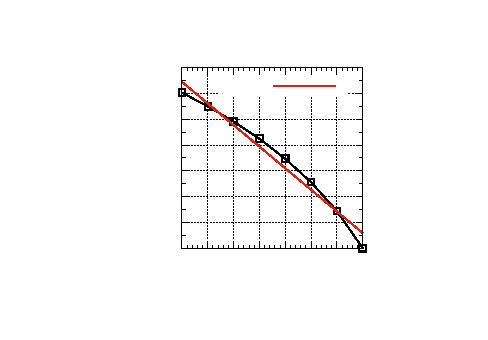
\includegraphics{kinetics/0/0b/mygraph}}%
    \gplfronttext
  \end{picture}%
\endgroup
\\[-3.5ex]
% GNUPLOT: LaTeX picture with Postscript
\begingroup
  \makeatletter
  \providecommand\color[2][]{%
    \GenericError{(gnuplot) \space\space\space\@spaces}{%
      Package color not loaded in conjunction with
      terminal option `colourtext'%
    }{See the gnuplot documentation for explanation.%
    }{Either use 'blacktext' in gnuplot or load the package
      color.sty in LaTeX.}%
    \renewcommand\color[2][]{}%
  }%
  \providecommand\includegraphics[2][]{%
    \GenericError{(gnuplot) \space\space\space\@spaces}{%
      Package graphicx or graphics not loaded%
    }{See the gnuplot documentation for explanation.%
    }{The gnuplot epslatex terminal needs graphicx.sty or graphics.sty.}%
    \renewcommand\includegraphics[2][]{}%
  }%
  \providecommand\rotatebox[2]{#2}%
  \@ifundefined{ifGPcolor}{%
    \newif\ifGPcolor
    \GPcolortrue
  }{}%
  \@ifundefined{ifGPblacktext}{%
    \newif\ifGPblacktext
    \GPblacktextfalse
  }{}%
  % define a \g@addto@macro without @ in the name:
  \let\gplgaddtomacro\g@addto@macro
  % define empty templates for all commands taking text:
  \gdef\gplbacktext{}%
  \gdef\gplfronttext{}%
  \makeatother
  \ifGPblacktext
    % no textcolor at all
    \def\colorrgb#1{}%
    \def\colorgray#1{}%
  \else
    % gray or color?
    \ifGPcolor
      \def\colorrgb#1{\color[rgb]{#1}}%
      \def\colorgray#1{\color[gray]{#1}}%
      \expandafter\def\csname LTw\endcsname{\color{white}}%
      \expandafter\def\csname LTb\endcsname{\color{black}}%
      \expandafter\def\csname LTa\endcsname{\color{black}}%
      \expandafter\def\csname LT0\endcsname{\color[rgb]{1,0,0}}%
      \expandafter\def\csname LT1\endcsname{\color[rgb]{0,1,0}}%
      \expandafter\def\csname LT2\endcsname{\color[rgb]{0,0,1}}%
      \expandafter\def\csname LT3\endcsname{\color[rgb]{1,0,1}}%
      \expandafter\def\csname LT4\endcsname{\color[rgb]{0,1,1}}%
      \expandafter\def\csname LT5\endcsname{\color[rgb]{1,1,0}}%
      \expandafter\def\csname LT6\endcsname{\color[rgb]{0,0,0}}%
      \expandafter\def\csname LT7\endcsname{\color[rgb]{1,0.3,0}}%
      \expandafter\def\csname LT8\endcsname{\color[rgb]{0.5,0.5,0.5}}%
    \else
      % gray
      \def\colorrgb#1{\color{black}}%
      \def\colorgray#1{\color[gray]{#1}}%
      \expandafter\def\csname LTw\endcsname{\color{white}}%
      \expandafter\def\csname LTb\endcsname{\color{black}}%
      \expandafter\def\csname LTa\endcsname{\color{black}}%
      \expandafter\def\csname LT0\endcsname{\color{black}}%
      \expandafter\def\csname LT1\endcsname{\color{black}}%
      \expandafter\def\csname LT2\endcsname{\color{black}}%
      \expandafter\def\csname LT3\endcsname{\color{black}}%
      \expandafter\def\csname LT4\endcsname{\color{black}}%
      \expandafter\def\csname LT5\endcsname{\color{black}}%
      \expandafter\def\csname LT6\endcsname{\color{black}}%
      \expandafter\def\csname LT7\endcsname{\color{black}}%
      \expandafter\def\csname LT8\endcsname{\color{black}}%
    \fi
  \fi
    \setlength{\unitlength}{0.0500bp}%
    \ifx\gptboxheight\undefined%
      \newlength{\gptboxheight}%
      \newlength{\gptboxwidth}%
      \newsavebox{\gptboxtext}%
    \fi%
    \setlength{\fboxrule}{0.5pt}%
    \setlength{\fboxsep}{1pt}%
\begin{picture}(4680.00,3276.00)%
    \gplgaddtomacro\gplbacktext{%
      \csname LTb\endcsname%%
      \put(1747,880){\makebox(0,0)[r]{\strut{}$0.005$}}%
      \csname LTb\endcsname%%
      \put(1747,1169){\makebox(0,0)[r]{\strut{}$0.01$}}%
      \csname LTb\endcsname%%
      \put(1747,1458){\makebox(0,0)[r]{\strut{}$0.015$}}%
      \csname LTb\endcsname%%
      \put(1747,1748){\makebox(0,0)[r]{\strut{}$0.02$}}%
      \csname LTb\endcsname%%
      \put(1747,2037){\makebox(0,0)[r]{\strut{}$0.025$}}%
      \csname LTb\endcsname%%
      \put(1747,2326){\makebox(0,0)[r]{\strut{}$0.03$}}%
      \csname LTb\endcsname%%
      \put(1747,2615){\makebox(0,0)[r]{\strut{}$0.035$}}%
      \csname LTb\endcsname%%
      \put(1879,660){\makebox(0,0){\strut{}$0$}}%
      \csname LTb\endcsname%%
      \put(2127,660){\makebox(0,0){\strut{}$1$}}%
      \csname LTb\endcsname%%
      \put(2375,660){\makebox(0,0){\strut{}$2$}}%
      \csname LTb\endcsname%%
      \put(2623,660){\makebox(0,0){\strut{}$3$}}%
      \csname LTb\endcsname%%
      \put(2870,660){\makebox(0,0){\strut{}$4$}}%
      \csname LTb\endcsname%%
      \put(3118,660){\makebox(0,0){\strut{}$5$}}%
      \csname LTb\endcsname%%
      \put(3366,660){\makebox(0,0){\strut{}$6$}}%
      \csname LTb\endcsname%%
      \put(3614,660){\makebox(0,0){\strut{}$7$}}%
    }%
    \gplgaddtomacro\gplfronttext{%
      \csname LTb\endcsname%%
      \put(867,1747){\rotatebox{-270}{\makebox(0,0){\strut{}1/(Concentration)}}}%
      \put(2746,330){\makebox(0,0){\strut{}Time (s)}}%
      \put(2746,2945){\makebox(0,0){\strut{}2nd Order Plot, $R^2$ = 0.89}}%
      \csname LTb\endcsname%%
      \put(2627,2442){\makebox(0,0)[r]{\strut{}fit}}%
    }%
    \gplbacktext
    \put(0,0){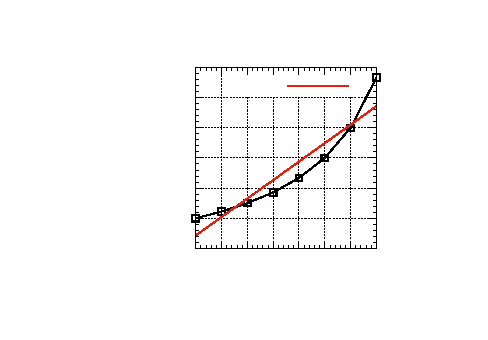
\includegraphics{kinetics/0/0c/mygraph}}%
    \gplfronttext
  \end{picture}%
\endgroup
\\}

\newpage

\begin{table}[H]
    \centering
    \caption{Kinetics Data --- 1st Order}
        \begin{tabular}{cSSS}
            \toprule
                Time & {Concentration} & {ln(Concentration)} & {1/(Concentration)} \\
                \midrule
                0     & 100   & 4.605 & 0.01 \\
                1     & 50    & 3.912 & 0.02 \\
                2     & 25    & 3.218 & 0.04 \\
                3     & 12.5  & 2.525 & 0.08 \\
                4     & 6.25  & 1.832 & 0.16 \\
                5     & 3.13  & 1.141 & 0.32 \\
                6     & 1.56  & 0.444 & 0.64 \\
                7     & 0.78  & -0.248 & 1.28 \\
            \bottomrule
        \end{tabular}
\end{table}
\vspace*{-.5cm}    
{\centering% GNUPLOT: LaTeX picture with Postscript
\begingroup
  \makeatletter
  \providecommand\color[2][]{%
    \GenericError{(gnuplot) \space\space\space\@spaces}{%
      Package color not loaded in conjunction with
      terminal option `colourtext'%
    }{See the gnuplot documentation for explanation.%
    }{Either use 'blacktext' in gnuplot or load the package
      color.sty in LaTeX.}%
    \renewcommand\color[2][]{}%
  }%
  \providecommand\includegraphics[2][]{%
    \GenericError{(gnuplot) \space\space\space\@spaces}{%
      Package graphicx or graphics not loaded%
    }{See the gnuplot documentation for explanation.%
    }{The gnuplot epslatex terminal needs graphicx.sty or graphics.sty.}%
    \renewcommand\includegraphics[2][]{}%
  }%
  \providecommand\rotatebox[2]{#2}%
  \@ifundefined{ifGPcolor}{%
    \newif\ifGPcolor
    \GPcolortrue
  }{}%
  \@ifundefined{ifGPblacktext}{%
    \newif\ifGPblacktext
    \GPblacktextfalse
  }{}%
  % define a \g@addto@macro without @ in the name:
  \let\gplgaddtomacro\g@addto@macro
  % define empty templates for all commands taking text:
  \gdef\gplbacktext{}%
  \gdef\gplfronttext{}%
  \makeatother
  \ifGPblacktext
    % no textcolor at all
    \def\colorrgb#1{}%
    \def\colorgray#1{}%
  \else
    % gray or color?
    \ifGPcolor
      \def\colorrgb#1{\color[rgb]{#1}}%
      \def\colorgray#1{\color[gray]{#1}}%
      \expandafter\def\csname LTw\endcsname{\color{white}}%
      \expandafter\def\csname LTb\endcsname{\color{black}}%
      \expandafter\def\csname LTa\endcsname{\color{black}}%
      \expandafter\def\csname LT0\endcsname{\color[rgb]{1,0,0}}%
      \expandafter\def\csname LT1\endcsname{\color[rgb]{0,1,0}}%
      \expandafter\def\csname LT2\endcsname{\color[rgb]{0,0,1}}%
      \expandafter\def\csname LT3\endcsname{\color[rgb]{1,0,1}}%
      \expandafter\def\csname LT4\endcsname{\color[rgb]{0,1,1}}%
      \expandafter\def\csname LT5\endcsname{\color[rgb]{1,1,0}}%
      \expandafter\def\csname LT6\endcsname{\color[rgb]{0,0,0}}%
      \expandafter\def\csname LT7\endcsname{\color[rgb]{1,0.3,0}}%
      \expandafter\def\csname LT8\endcsname{\color[rgb]{0.5,0.5,0.5}}%
    \else
      % gray
      \def\colorrgb#1{\color{black}}%
      \def\colorgray#1{\color[gray]{#1}}%
      \expandafter\def\csname LTw\endcsname{\color{white}}%
      \expandafter\def\csname LTb\endcsname{\color{black}}%
      \expandafter\def\csname LTa\endcsname{\color{black}}%
      \expandafter\def\csname LT0\endcsname{\color{black}}%
      \expandafter\def\csname LT1\endcsname{\color{black}}%
      \expandafter\def\csname LT2\endcsname{\color{black}}%
      \expandafter\def\csname LT3\endcsname{\color{black}}%
      \expandafter\def\csname LT4\endcsname{\color{black}}%
      \expandafter\def\csname LT5\endcsname{\color{black}}%
      \expandafter\def\csname LT6\endcsname{\color{black}}%
      \expandafter\def\csname LT7\endcsname{\color{black}}%
      \expandafter\def\csname LT8\endcsname{\color{black}}%
    \fi
  \fi
    \setlength{\unitlength}{0.0500bp}%
    \ifx\gptboxheight\undefined%
      \newlength{\gptboxheight}%
      \newlength{\gptboxwidth}%
      \newsavebox{\gptboxtext}%
    \fi%
    \setlength{\fboxrule}{0.5pt}%
    \setlength{\fboxsep}{1pt}%
\begin{picture}(4680.00,3276.00)%
    \gplgaddtomacro\gplbacktext{%
      \csname LTb\endcsname%%
      \put(1615,880){\makebox(0,0)[r]{\strut{}$-20$}}%
      \csname LTb\endcsname%%
      \put(1615,1169){\makebox(0,0)[r]{\strut{}$0$}}%
      \csname LTb\endcsname%%
      \put(1615,1458){\makebox(0,0)[r]{\strut{}$20$}}%
      \csname LTb\endcsname%%
      \put(1615,1748){\makebox(0,0)[r]{\strut{}$40$}}%
      \csname LTb\endcsname%%
      \put(1615,2037){\makebox(0,0)[r]{\strut{}$60$}}%
      \csname LTb\endcsname%%
      \put(1615,2326){\makebox(0,0)[r]{\strut{}$80$}}%
      \csname LTb\endcsname%%
      \put(1615,2615){\makebox(0,0)[r]{\strut{}$100$}}%
      \csname LTb\endcsname%%
      \put(1747,660){\makebox(0,0){\strut{}$0$}}%
      \csname LTb\endcsname%%
      \put(1995,660){\makebox(0,0){\strut{}$1$}}%
      \csname LTb\endcsname%%
      \put(2243,660){\makebox(0,0){\strut{}$2$}}%
      \csname LTb\endcsname%%
      \put(2491,660){\makebox(0,0){\strut{}$3$}}%
      \csname LTb\endcsname%%
      \put(2738,660){\makebox(0,0){\strut{}$4$}}%
      \csname LTb\endcsname%%
      \put(2986,660){\makebox(0,0){\strut{}$5$}}%
      \csname LTb\endcsname%%
      \put(3234,660){\makebox(0,0){\strut{}$6$}}%
      \csname LTb\endcsname%%
      \put(3482,660){\makebox(0,0){\strut{}$7$}}%
    }%
    \gplgaddtomacro\gplfronttext{%
      \csname LTb\endcsname%%
      \put(999,1747){\rotatebox{-270}{\makebox(0,0){\strut{}Concentration}}}%
      \put(2614,330){\makebox(0,0){\strut{}Time (s)}}%
      \put(2614,2945){\makebox(0,0){\strut{}0th Order Plot, $R^2$ = 0.73}}%
      \csname LTb\endcsname%%
      \put(2495,2442){\makebox(0,0)[r]{\strut{}fit}}%
    }%
    \gplbacktext
    \put(0,0){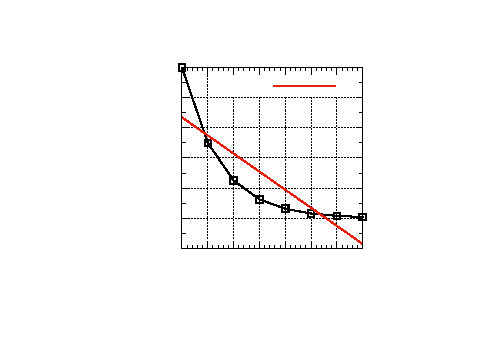
\includegraphics{kinetics/1/1a/mygraph}}%
    \gplfronttext
  \end{picture}%
\endgroup
\\[-3.5ex]
% GNUPLOT: LaTeX picture with Postscript
\begingroup
  \makeatletter
  \providecommand\color[2][]{%
    \GenericError{(gnuplot) \space\space\space\@spaces}{%
      Package color not loaded in conjunction with
      terminal option `colourtext'%
    }{See the gnuplot documentation for explanation.%
    }{Either use 'blacktext' in gnuplot or load the package
      color.sty in LaTeX.}%
    \renewcommand\color[2][]{}%
  }%
  \providecommand\includegraphics[2][]{%
    \GenericError{(gnuplot) \space\space\space\@spaces}{%
      Package graphicx or graphics not loaded%
    }{See the gnuplot documentation for explanation.%
    }{The gnuplot epslatex terminal needs graphicx.sty or graphics.sty.}%
    \renewcommand\includegraphics[2][]{}%
  }%
  \providecommand\rotatebox[2]{#2}%
  \@ifundefined{ifGPcolor}{%
    \newif\ifGPcolor
    \GPcolortrue
  }{}%
  \@ifundefined{ifGPblacktext}{%
    \newif\ifGPblacktext
    \GPblacktextfalse
  }{}%
  % define a \g@addto@macro without @ in the name:
  \let\gplgaddtomacro\g@addto@macro
  % define empty templates for all commands taking text:
  \gdef\gplbacktext{}%
  \gdef\gplfronttext{}%
  \makeatother
  \ifGPblacktext
    % no textcolor at all
    \def\colorrgb#1{}%
    \def\colorgray#1{}%
  \else
    % gray or color?
    \ifGPcolor
      \def\colorrgb#1{\color[rgb]{#1}}%
      \def\colorgray#1{\color[gray]{#1}}%
      \expandafter\def\csname LTw\endcsname{\color{white}}%
      \expandafter\def\csname LTb\endcsname{\color{black}}%
      \expandafter\def\csname LTa\endcsname{\color{black}}%
      \expandafter\def\csname LT0\endcsname{\color[rgb]{1,0,0}}%
      \expandafter\def\csname LT1\endcsname{\color[rgb]{0,1,0}}%
      \expandafter\def\csname LT2\endcsname{\color[rgb]{0,0,1}}%
      \expandafter\def\csname LT3\endcsname{\color[rgb]{1,0,1}}%
      \expandafter\def\csname LT4\endcsname{\color[rgb]{0,1,1}}%
      \expandafter\def\csname LT5\endcsname{\color[rgb]{1,1,0}}%
      \expandafter\def\csname LT6\endcsname{\color[rgb]{0,0,0}}%
      \expandafter\def\csname LT7\endcsname{\color[rgb]{1,0.3,0}}%
      \expandafter\def\csname LT8\endcsname{\color[rgb]{0.5,0.5,0.5}}%
    \else
      % gray
      \def\colorrgb#1{\color{black}}%
      \def\colorgray#1{\color[gray]{#1}}%
      \expandafter\def\csname LTw\endcsname{\color{white}}%
      \expandafter\def\csname LTb\endcsname{\color{black}}%
      \expandafter\def\csname LTa\endcsname{\color{black}}%
      \expandafter\def\csname LT0\endcsname{\color{black}}%
      \expandafter\def\csname LT1\endcsname{\color{black}}%
      \expandafter\def\csname LT2\endcsname{\color{black}}%
      \expandafter\def\csname LT3\endcsname{\color{black}}%
      \expandafter\def\csname LT4\endcsname{\color{black}}%
      \expandafter\def\csname LT5\endcsname{\color{black}}%
      \expandafter\def\csname LT6\endcsname{\color{black}}%
      \expandafter\def\csname LT7\endcsname{\color{black}}%
      \expandafter\def\csname LT8\endcsname{\color{black}}%
    \fi
  \fi
    \setlength{\unitlength}{0.0500bp}%
    \ifx\gptboxheight\undefined%
      \newlength{\gptboxheight}%
      \newlength{\gptboxwidth}%
      \newsavebox{\gptboxtext}%
    \fi%
    \setlength{\fboxrule}{0.5pt}%
    \setlength{\fboxsep}{1pt}%
\begin{picture}(4680.00,3276.00)%
    \gplgaddtomacro\gplbacktext{%
      \csname LTb\endcsname%%
      \put(1681,880){\makebox(0,0)[r]{\strut{}$-0.5$}}%
      \csname LTb\endcsname%%
      \put(1681,1038){\makebox(0,0)[r]{\strut{}$0$}}%
      \csname LTb\endcsname%%
      \put(1681,1195){\makebox(0,0)[r]{\strut{}$0.5$}}%
      \csname LTb\endcsname%%
      \put(1681,1353){\makebox(0,0)[r]{\strut{}$1$}}%
      \csname LTb\endcsname%%
      \put(1681,1511){\makebox(0,0)[r]{\strut{}$1.5$}}%
      \csname LTb\endcsname%%
      \put(1681,1669){\makebox(0,0)[r]{\strut{}$2$}}%
      \csname LTb\endcsname%%
      \put(1681,1826){\makebox(0,0)[r]{\strut{}$2.5$}}%
      \csname LTb\endcsname%%
      \put(1681,1984){\makebox(0,0)[r]{\strut{}$3$}}%
      \csname LTb\endcsname%%
      \put(1681,2142){\makebox(0,0)[r]{\strut{}$3.5$}}%
      \csname LTb\endcsname%%
      \put(1681,2300){\makebox(0,0)[r]{\strut{}$4$}}%
      \csname LTb\endcsname%%
      \put(1681,2457){\makebox(0,0)[r]{\strut{}$4.5$}}%
      \csname LTb\endcsname%%
      \put(1681,2615){\makebox(0,0)[r]{\strut{}$5$}}%
      \csname LTb\endcsname%%
      \put(1813,660){\makebox(0,0){\strut{}$0$}}%
      \csname LTb\endcsname%%
      \put(2061,660){\makebox(0,0){\strut{}$1$}}%
      \csname LTb\endcsname%%
      \put(2309,660){\makebox(0,0){\strut{}$2$}}%
      \csname LTb\endcsname%%
      \put(2557,660){\makebox(0,0){\strut{}$3$}}%
      \csname LTb\endcsname%%
      \put(2804,660){\makebox(0,0){\strut{}$4$}}%
      \csname LTb\endcsname%%
      \put(3052,660){\makebox(0,0){\strut{}$5$}}%
      \csname LTb\endcsname%%
      \put(3300,660){\makebox(0,0){\strut{}$6$}}%
      \csname LTb\endcsname%%
      \put(3548,660){\makebox(0,0){\strut{}$7$}}%
    }%
    \gplgaddtomacro\gplfronttext{%
      \csname LTb\endcsname%%
      \put(933,1747){\rotatebox{-270}{\makebox(0,0){\strut{}ln(Concentration)}}}%
      \put(2680,330){\makebox(0,0){\strut{}Time (s)}}%
      \put(2680,2945){\makebox(0,0){\strut{}1st Order Plot, $R^2$ = 1}}%
      \csname LTb\endcsname%%
      \put(2561,2442){\makebox(0,0)[r]{\strut{}fit}}%
    }%
    \gplbacktext
    \put(0,0){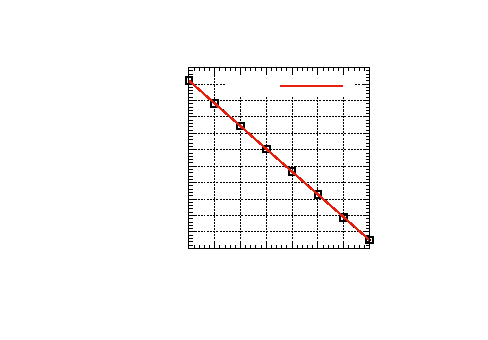
\includegraphics{kinetics/1/1b/mygraph}}%
    \gplfronttext
  \end{picture}%
\endgroup
\\[-3.5ex]
% GNUPLOT: LaTeX picture with Postscript
\begingroup
  \makeatletter
  \providecommand\color[2][]{%
    \GenericError{(gnuplot) \space\space\space\@spaces}{%
      Package color not loaded in conjunction with
      terminal option `colourtext'%
    }{See the gnuplot documentation for explanation.%
    }{Either use 'blacktext' in gnuplot or load the package
      color.sty in LaTeX.}%
    \renewcommand\color[2][]{}%
  }%
  \providecommand\includegraphics[2][]{%
    \GenericError{(gnuplot) \space\space\space\@spaces}{%
      Package graphicx or graphics not loaded%
    }{See the gnuplot documentation for explanation.%
    }{The gnuplot epslatex terminal needs graphicx.sty or graphics.sty.}%
    \renewcommand\includegraphics[2][]{}%
  }%
  \providecommand\rotatebox[2]{#2}%
  \@ifundefined{ifGPcolor}{%
    \newif\ifGPcolor
    \GPcolortrue
  }{}%
  \@ifundefined{ifGPblacktext}{%
    \newif\ifGPblacktext
    \GPblacktextfalse
  }{}%
  % define a \g@addto@macro without @ in the name:
  \let\gplgaddtomacro\g@addto@macro
  % define empty templates for all commands taking text:
  \gdef\gplbacktext{}%
  \gdef\gplfronttext{}%
  \makeatother
  \ifGPblacktext
    % no textcolor at all
    \def\colorrgb#1{}%
    \def\colorgray#1{}%
  \else
    % gray or color?
    \ifGPcolor
      \def\colorrgb#1{\color[rgb]{#1}}%
      \def\colorgray#1{\color[gray]{#1}}%
      \expandafter\def\csname LTw\endcsname{\color{white}}%
      \expandafter\def\csname LTb\endcsname{\color{black}}%
      \expandafter\def\csname LTa\endcsname{\color{black}}%
      \expandafter\def\csname LT0\endcsname{\color[rgb]{1,0,0}}%
      \expandafter\def\csname LT1\endcsname{\color[rgb]{0,1,0}}%
      \expandafter\def\csname LT2\endcsname{\color[rgb]{0,0,1}}%
      \expandafter\def\csname LT3\endcsname{\color[rgb]{1,0,1}}%
      \expandafter\def\csname LT4\endcsname{\color[rgb]{0,1,1}}%
      \expandafter\def\csname LT5\endcsname{\color[rgb]{1,1,0}}%
      \expandafter\def\csname LT6\endcsname{\color[rgb]{0,0,0}}%
      \expandafter\def\csname LT7\endcsname{\color[rgb]{1,0.3,0}}%
      \expandafter\def\csname LT8\endcsname{\color[rgb]{0.5,0.5,0.5}}%
    \else
      % gray
      \def\colorrgb#1{\color{black}}%
      \def\colorgray#1{\color[gray]{#1}}%
      \expandafter\def\csname LTw\endcsname{\color{white}}%
      \expandafter\def\csname LTb\endcsname{\color{black}}%
      \expandafter\def\csname LTa\endcsname{\color{black}}%
      \expandafter\def\csname LT0\endcsname{\color{black}}%
      \expandafter\def\csname LT1\endcsname{\color{black}}%
      \expandafter\def\csname LT2\endcsname{\color{black}}%
      \expandafter\def\csname LT3\endcsname{\color{black}}%
      \expandafter\def\csname LT4\endcsname{\color{black}}%
      \expandafter\def\csname LT5\endcsname{\color{black}}%
      \expandafter\def\csname LT6\endcsname{\color{black}}%
      \expandafter\def\csname LT7\endcsname{\color{black}}%
      \expandafter\def\csname LT8\endcsname{\color{black}}%
    \fi
  \fi
    \setlength{\unitlength}{0.0500bp}%
    \ifx\gptboxheight\undefined%
      \newlength{\gptboxheight}%
      \newlength{\gptboxwidth}%
      \newsavebox{\gptboxtext}%
    \fi%
    \setlength{\fboxrule}{0.5pt}%
    \setlength{\fboxsep}{1pt}%
\begin{picture}(4680.00,3276.00)%
    \gplgaddtomacro\gplbacktext{%
      \csname LTb\endcsname%%
      \put(1681,880){\makebox(0,0)[r]{\strut{}$-0.4$}}%
      \csname LTb\endcsname%%
      \put(1681,1073){\makebox(0,0)[r]{\strut{}$-0.2$}}%
      \csname LTb\endcsname%%
      \put(1681,1266){\makebox(0,0)[r]{\strut{}$0$}}%
      \csname LTb\endcsname%%
      \put(1681,1458){\makebox(0,0)[r]{\strut{}$0.2$}}%
      \csname LTb\endcsname%%
      \put(1681,1651){\makebox(0,0)[r]{\strut{}$0.4$}}%
      \csname LTb\endcsname%%
      \put(1681,1844){\makebox(0,0)[r]{\strut{}$0.6$}}%
      \csname LTb\endcsname%%
      \put(1681,2037){\makebox(0,0)[r]{\strut{}$0.8$}}%
      \csname LTb\endcsname%%
      \put(1681,2229){\makebox(0,0)[r]{\strut{}$1$}}%
      \csname LTb\endcsname%%
      \put(1681,2422){\makebox(0,0)[r]{\strut{}$1.2$}}%
      \csname LTb\endcsname%%
      \put(1681,2615){\makebox(0,0)[r]{\strut{}$1.4$}}%
      \csname LTb\endcsname%%
      \put(1813,660){\makebox(0,0){\strut{}$0$}}%
      \csname LTb\endcsname%%
      \put(2061,660){\makebox(0,0){\strut{}$1$}}%
      \csname LTb\endcsname%%
      \put(2309,660){\makebox(0,0){\strut{}$2$}}%
      \csname LTb\endcsname%%
      \put(2557,660){\makebox(0,0){\strut{}$3$}}%
      \csname LTb\endcsname%%
      \put(2804,660){\makebox(0,0){\strut{}$4$}}%
      \csname LTb\endcsname%%
      \put(3052,660){\makebox(0,0){\strut{}$5$}}%
      \csname LTb\endcsname%%
      \put(3300,660){\makebox(0,0){\strut{}$6$}}%
      \csname LTb\endcsname%%
      \put(3548,660){\makebox(0,0){\strut{}$7$}}%
    }%
    \gplgaddtomacro\gplfronttext{%
      \csname LTb\endcsname%%
      \put(933,1747){\rotatebox{-270}{\makebox(0,0){\strut{}1/(Concentration)}}}%
      \put(2680,330){\makebox(0,0){\strut{}Time (s)}}%
      \put(2680,2945){\makebox(0,0){\strut{}2nd Order Plot, $R^2$ = 0.72}}%
      \csname LTb\endcsname%%
      \put(2561,2442){\makebox(0,0)[r]{\strut{}fit}}%
    }%
    \gplbacktext
    \put(0,0){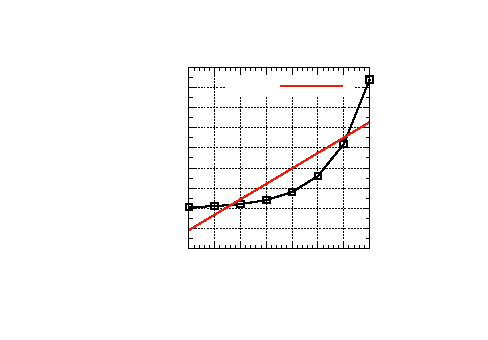
\includegraphics{kinetics/1/1c/mygraph}}%
    \gplfronttext
  \end{picture}%
\endgroup
\\}

\newpage
\begin{table}[htbp]
    \centering
    \caption{Kinetics Data --- 2nd Order}
        \begin{tabular}{cScc}
            \toprule
                Time & {Concentration} & ln(Concentration) & 1/(Concentration) \\
                \midrule
                0     & 100   & 4.605 & 0.01 \\
                1     & 50    & 3.912 & 0.02 \\
                2     & 33.3  & 3.505 & 0.03 \\
                3     & 25    & 3.218 & 0.04 \\
                4     & 20    & 2.995 & 0.05 \\
                5     & 16.67 & 2.813 & 0.06 \\
                6     & 14.28 & 2.658 & 0.07 \\
                7     & 12.5  & 2.525 & 0.08 \\
            \bottomrule
        \end{tabular}
\end{table}
\vspace*{-.5cm}    
{\centering% GNUPLOT: LaTeX picture with Postscript
\begingroup
  \makeatletter
  \providecommand\color[2][]{%
    \GenericError{(gnuplot) \space\space\space\@spaces}{%
      Package color not loaded in conjunction with
      terminal option `colourtext'%
    }{See the gnuplot documentation for explanation.%
    }{Either use 'blacktext' in gnuplot or load the package
      color.sty in LaTeX.}%
    \renewcommand\color[2][]{}%
  }%
  \providecommand\includegraphics[2][]{%
    \GenericError{(gnuplot) \space\space\space\@spaces}{%
      Package graphicx or graphics not loaded%
    }{See the gnuplot documentation for explanation.%
    }{The gnuplot epslatex terminal needs graphicx.sty or graphics.sty.}%
    \renewcommand\includegraphics[2][]{}%
  }%
  \providecommand\rotatebox[2]{#2}%
  \@ifundefined{ifGPcolor}{%
    \newif\ifGPcolor
    \GPcolortrue
  }{}%
  \@ifundefined{ifGPblacktext}{%
    \newif\ifGPblacktext
    \GPblacktextfalse
  }{}%
  % define a \g@addto@macro without @ in the name:
  \let\gplgaddtomacro\g@addto@macro
  % define empty templates for all commands taking text:
  \gdef\gplbacktext{}%
  \gdef\gplfronttext{}%
  \makeatother
  \ifGPblacktext
    % no textcolor at all
    \def\colorrgb#1{}%
    \def\colorgray#1{}%
  \else
    % gray or color?
    \ifGPcolor
      \def\colorrgb#1{\color[rgb]{#1}}%
      \def\colorgray#1{\color[gray]{#1}}%
      \expandafter\def\csname LTw\endcsname{\color{white}}%
      \expandafter\def\csname LTb\endcsname{\color{black}}%
      \expandafter\def\csname LTa\endcsname{\color{black}}%
      \expandafter\def\csname LT0\endcsname{\color[rgb]{1,0,0}}%
      \expandafter\def\csname LT1\endcsname{\color[rgb]{0,1,0}}%
      \expandafter\def\csname LT2\endcsname{\color[rgb]{0,0,1}}%
      \expandafter\def\csname LT3\endcsname{\color[rgb]{1,0,1}}%
      \expandafter\def\csname LT4\endcsname{\color[rgb]{0,1,1}}%
      \expandafter\def\csname LT5\endcsname{\color[rgb]{1,1,0}}%
      \expandafter\def\csname LT6\endcsname{\color[rgb]{0,0,0}}%
      \expandafter\def\csname LT7\endcsname{\color[rgb]{1,0.3,0}}%
      \expandafter\def\csname LT8\endcsname{\color[rgb]{0.5,0.5,0.5}}%
    \else
      % gray
      \def\colorrgb#1{\color{black}}%
      \def\colorgray#1{\color[gray]{#1}}%
      \expandafter\def\csname LTw\endcsname{\color{white}}%
      \expandafter\def\csname LTb\endcsname{\color{black}}%
      \expandafter\def\csname LTa\endcsname{\color{black}}%
      \expandafter\def\csname LT0\endcsname{\color{black}}%
      \expandafter\def\csname LT1\endcsname{\color{black}}%
      \expandafter\def\csname LT2\endcsname{\color{black}}%
      \expandafter\def\csname LT3\endcsname{\color{black}}%
      \expandafter\def\csname LT4\endcsname{\color{black}}%
      \expandafter\def\csname LT5\endcsname{\color{black}}%
      \expandafter\def\csname LT6\endcsname{\color{black}}%
      \expandafter\def\csname LT7\endcsname{\color{black}}%
      \expandafter\def\csname LT8\endcsname{\color{black}}%
    \fi
  \fi
    \setlength{\unitlength}{0.0500bp}%
    \ifx\gptboxheight\undefined%
      \newlength{\gptboxheight}%
      \newlength{\gptboxwidth}%
      \newsavebox{\gptboxtext}%
    \fi%
    \setlength{\fboxrule}{0.5pt}%
    \setlength{\fboxsep}{1pt}%
\begin{picture}(4680.00,3276.00)%
    \gplgaddtomacro\gplbacktext{%
      \csname LTb\endcsname%%
      \put(1615,880){\makebox(0,0)[r]{\strut{}$0$}}%
      \csname LTb\endcsname%%
      \put(1615,1227){\makebox(0,0)[r]{\strut{}$20$}}%
      \csname LTb\endcsname%%
      \put(1615,1574){\makebox(0,0)[r]{\strut{}$40$}}%
      \csname LTb\endcsname%%
      \put(1615,1921){\makebox(0,0)[r]{\strut{}$60$}}%
      \csname LTb\endcsname%%
      \put(1615,2268){\makebox(0,0)[r]{\strut{}$80$}}%
      \csname LTb\endcsname%%
      \put(1615,2615){\makebox(0,0)[r]{\strut{}$100$}}%
      \csname LTb\endcsname%%
      \put(1747,660){\makebox(0,0){\strut{}$0$}}%
      \csname LTb\endcsname%%
      \put(1995,660){\makebox(0,0){\strut{}$1$}}%
      \csname LTb\endcsname%%
      \put(2243,660){\makebox(0,0){\strut{}$2$}}%
      \csname LTb\endcsname%%
      \put(2491,660){\makebox(0,0){\strut{}$3$}}%
      \csname LTb\endcsname%%
      \put(2738,660){\makebox(0,0){\strut{}$4$}}%
      \csname LTb\endcsname%%
      \put(2986,660){\makebox(0,0){\strut{}$5$}}%
      \csname LTb\endcsname%%
      \put(3234,660){\makebox(0,0){\strut{}$6$}}%
      \csname LTb\endcsname%%
      \put(3482,660){\makebox(0,0){\strut{}$7$}}%
    }%
    \gplgaddtomacro\gplfronttext{%
      \csname LTb\endcsname%%
      \put(999,1747){\rotatebox{-270}{\makebox(0,0){\strut{}Concentration}}}%
      \put(2614,330){\makebox(0,0){\strut{}Time (s)}}%
      \put(2614,2945){\makebox(0,0){\strut{}0th Order Plot, $R^2$ = 0.70}}%
      \csname LTb\endcsname%%
      \put(2495,2442){\makebox(0,0)[r]{\strut{}fit}}%
    }%
    \gplbacktext
    \put(0,0){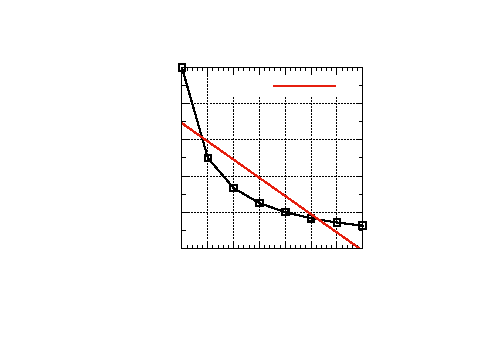
\includegraphics{kinetics/2/2a/mygraph}}%
    \gplfronttext
  \end{picture}%
\endgroup
\\[-3.5ex]
% GNUPLOT: LaTeX picture with Postscript
\begingroup
  \makeatletter
  \providecommand\color[2][]{%
    \GenericError{(gnuplot) \space\space\space\@spaces}{%
      Package color not loaded in conjunction with
      terminal option `colourtext'%
    }{See the gnuplot documentation for explanation.%
    }{Either use 'blacktext' in gnuplot or load the package
      color.sty in LaTeX.}%
    \renewcommand\color[2][]{}%
  }%
  \providecommand\includegraphics[2][]{%
    \GenericError{(gnuplot) \space\space\space\@spaces}{%
      Package graphicx or graphics not loaded%
    }{See the gnuplot documentation for explanation.%
    }{The gnuplot epslatex terminal needs graphicx.sty or graphics.sty.}%
    \renewcommand\includegraphics[2][]{}%
  }%
  \providecommand\rotatebox[2]{#2}%
  \@ifundefined{ifGPcolor}{%
    \newif\ifGPcolor
    \GPcolortrue
  }{}%
  \@ifundefined{ifGPblacktext}{%
    \newif\ifGPblacktext
    \GPblacktextfalse
  }{}%
  % define a \g@addto@macro without @ in the name:
  \let\gplgaddtomacro\g@addto@macro
  % define empty templates for all commands taking text:
  \gdef\gplbacktext{}%
  \gdef\gplfronttext{}%
  \makeatother
  \ifGPblacktext
    % no textcolor at all
    \def\colorrgb#1{}%
    \def\colorgray#1{}%
  \else
    % gray or color?
    \ifGPcolor
      \def\colorrgb#1{\color[rgb]{#1}}%
      \def\colorgray#1{\color[gray]{#1}}%
      \expandafter\def\csname LTw\endcsname{\color{white}}%
      \expandafter\def\csname LTb\endcsname{\color{black}}%
      \expandafter\def\csname LTa\endcsname{\color{black}}%
      \expandafter\def\csname LT0\endcsname{\color[rgb]{1,0,0}}%
      \expandafter\def\csname LT1\endcsname{\color[rgb]{0,1,0}}%
      \expandafter\def\csname LT2\endcsname{\color[rgb]{0,0,1}}%
      \expandafter\def\csname LT3\endcsname{\color[rgb]{1,0,1}}%
      \expandafter\def\csname LT4\endcsname{\color[rgb]{0,1,1}}%
      \expandafter\def\csname LT5\endcsname{\color[rgb]{1,1,0}}%
      \expandafter\def\csname LT6\endcsname{\color[rgb]{0,0,0}}%
      \expandafter\def\csname LT7\endcsname{\color[rgb]{1,0.3,0}}%
      \expandafter\def\csname LT8\endcsname{\color[rgb]{0.5,0.5,0.5}}%
    \else
      % gray
      \def\colorrgb#1{\color{black}}%
      \def\colorgray#1{\color[gray]{#1}}%
      \expandafter\def\csname LTw\endcsname{\color{white}}%
      \expandafter\def\csname LTb\endcsname{\color{black}}%
      \expandafter\def\csname LTa\endcsname{\color{black}}%
      \expandafter\def\csname LT0\endcsname{\color{black}}%
      \expandafter\def\csname LT1\endcsname{\color{black}}%
      \expandafter\def\csname LT2\endcsname{\color{black}}%
      \expandafter\def\csname LT3\endcsname{\color{black}}%
      \expandafter\def\csname LT4\endcsname{\color{black}}%
      \expandafter\def\csname LT5\endcsname{\color{black}}%
      \expandafter\def\csname LT6\endcsname{\color{black}}%
      \expandafter\def\csname LT7\endcsname{\color{black}}%
      \expandafter\def\csname LT8\endcsname{\color{black}}%
    \fi
  \fi
    \setlength{\unitlength}{0.0500bp}%
    \ifx\gptboxheight\undefined%
      \newlength{\gptboxheight}%
      \newlength{\gptboxwidth}%
      \newsavebox{\gptboxtext}%
    \fi%
    \setlength{\fboxrule}{0.5pt}%
    \setlength{\fboxsep}{1pt}%
\begin{picture}(4680.00,3276.00)%
    \gplgaddtomacro\gplbacktext{%
      \csname LTb\endcsname%%
      \put(1615,880){\makebox(0,0)[r]{\strut{}$2$}}%
      \csname LTb\endcsname%%
      \put(1615,1169){\makebox(0,0)[r]{\strut{}$2.5$}}%
      \csname LTb\endcsname%%
      \put(1615,1458){\makebox(0,0)[r]{\strut{}$3$}}%
      \csname LTb\endcsname%%
      \put(1615,1748){\makebox(0,0)[r]{\strut{}$3.5$}}%
      \csname LTb\endcsname%%
      \put(1615,2037){\makebox(0,0)[r]{\strut{}$4$}}%
      \csname LTb\endcsname%%
      \put(1615,2326){\makebox(0,0)[r]{\strut{}$4.5$}}%
      \csname LTb\endcsname%%
      \put(1615,2615){\makebox(0,0)[r]{\strut{}$5$}}%
      \csname LTb\endcsname%%
      \put(1747,660){\makebox(0,0){\strut{}$0$}}%
      \csname LTb\endcsname%%
      \put(1995,660){\makebox(0,0){\strut{}$1$}}%
      \csname LTb\endcsname%%
      \put(2243,660){\makebox(0,0){\strut{}$2$}}%
      \csname LTb\endcsname%%
      \put(2491,660){\makebox(0,0){\strut{}$3$}}%
      \csname LTb\endcsname%%
      \put(2738,660){\makebox(0,0){\strut{}$4$}}%
      \csname LTb\endcsname%%
      \put(2986,660){\makebox(0,0){\strut{}$5$}}%
      \csname LTb\endcsname%%
      \put(3234,660){\makebox(0,0){\strut{}$6$}}%
      \csname LTb\endcsname%%
      \put(3482,660){\makebox(0,0){\strut{}$7$}}%
    }%
    \gplgaddtomacro\gplfronttext{%
      \csname LTb\endcsname%%
      \put(999,1747){\rotatebox{-270}{\makebox(0,0){\strut{}ln(Concentration)}}}%
      \put(2614,330){\makebox(0,0){\strut{}Time (s)}}%
      \put(2614,2945){\makebox(0,0){\strut{}1st Order Plot, $R^2$ = 0.92}}%
      \csname LTb\endcsname%%
      \put(2495,2442){\makebox(0,0)[r]{\strut{}fit}}%
    }%
    \gplbacktext
    \put(0,0){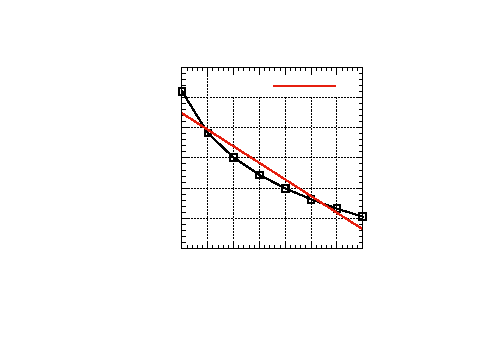
\includegraphics{kinetics/2/2b/mygraph}}%
    \gplfronttext
  \end{picture}%
\endgroup
\\[-3.5ex]
% GNUPLOT: LaTeX picture with Postscript
\begingroup
  \makeatletter
  \providecommand\color[2][]{%
    \GenericError{(gnuplot) \space\space\space\@spaces}{%
      Package color not loaded in conjunction with
      terminal option `colourtext'%
    }{See the gnuplot documentation for explanation.%
    }{Either use 'blacktext' in gnuplot or load the package
      color.sty in LaTeX.}%
    \renewcommand\color[2][]{}%
  }%
  \providecommand\includegraphics[2][]{%
    \GenericError{(gnuplot) \space\space\space\@spaces}{%
      Package graphicx or graphics not loaded%
    }{See the gnuplot documentation for explanation.%
    }{The gnuplot epslatex terminal needs graphicx.sty or graphics.sty.}%
    \renewcommand\includegraphics[2][]{}%
  }%
  \providecommand\rotatebox[2]{#2}%
  \@ifundefined{ifGPcolor}{%
    \newif\ifGPcolor
    \GPcolortrue
  }{}%
  \@ifundefined{ifGPblacktext}{%
    \newif\ifGPblacktext
    \GPblacktextfalse
  }{}%
  % define a \g@addto@macro without @ in the name:
  \let\gplgaddtomacro\g@addto@macro
  % define empty templates for all commands taking text:
  \gdef\gplbacktext{}%
  \gdef\gplfronttext{}%
  \makeatother
  \ifGPblacktext
    % no textcolor at all
    \def\colorrgb#1{}%
    \def\colorgray#1{}%
  \else
    % gray or color?
    \ifGPcolor
      \def\colorrgb#1{\color[rgb]{#1}}%
      \def\colorgray#1{\color[gray]{#1}}%
      \expandafter\def\csname LTw\endcsname{\color{white}}%
      \expandafter\def\csname LTb\endcsname{\color{black}}%
      \expandafter\def\csname LTa\endcsname{\color{black}}%
      \expandafter\def\csname LT0\endcsname{\color[rgb]{1,0,0}}%
      \expandafter\def\csname LT1\endcsname{\color[rgb]{0,1,0}}%
      \expandafter\def\csname LT2\endcsname{\color[rgb]{0,0,1}}%
      \expandafter\def\csname LT3\endcsname{\color[rgb]{1,0,1}}%
      \expandafter\def\csname LT4\endcsname{\color[rgb]{0,1,1}}%
      \expandafter\def\csname LT5\endcsname{\color[rgb]{1,1,0}}%
      \expandafter\def\csname LT6\endcsname{\color[rgb]{0,0,0}}%
      \expandafter\def\csname LT7\endcsname{\color[rgb]{1,0.3,0}}%
      \expandafter\def\csname LT8\endcsname{\color[rgb]{0.5,0.5,0.5}}%
    \else
      % gray
      \def\colorrgb#1{\color{black}}%
      \def\colorgray#1{\color[gray]{#1}}%
      \expandafter\def\csname LTw\endcsname{\color{white}}%
      \expandafter\def\csname LTb\endcsname{\color{black}}%
      \expandafter\def\csname LTa\endcsname{\color{black}}%
      \expandafter\def\csname LT0\endcsname{\color{black}}%
      \expandafter\def\csname LT1\endcsname{\color{black}}%
      \expandafter\def\csname LT2\endcsname{\color{black}}%
      \expandafter\def\csname LT3\endcsname{\color{black}}%
      \expandafter\def\csname LT4\endcsname{\color{black}}%
      \expandafter\def\csname LT5\endcsname{\color{black}}%
      \expandafter\def\csname LT6\endcsname{\color{black}}%
      \expandafter\def\csname LT7\endcsname{\color{black}}%
      \expandafter\def\csname LT8\endcsname{\color{black}}%
    \fi
  \fi
    \setlength{\unitlength}{0.0500bp}%
    \ifx\gptboxheight\undefined%
      \newlength{\gptboxheight}%
      \newlength{\gptboxwidth}%
      \newsavebox{\gptboxtext}%
    \fi%
    \setlength{\fboxrule}{0.5pt}%
    \setlength{\fboxsep}{1pt}%
\begin{picture}(4680.00,3276.00)%
    \gplgaddtomacro\gplbacktext{%
      \csname LTb\endcsname%%
      \put(1681,880){\makebox(0,0)[r]{\strut{}$0.01$}}%
      \csname LTb\endcsname%%
      \put(1681,1097){\makebox(0,0)[r]{\strut{}$0.02$}}%
      \csname LTb\endcsname%%
      \put(1681,1314){\makebox(0,0)[r]{\strut{}$0.03$}}%
      \csname LTb\endcsname%%
      \put(1681,1531){\makebox(0,0)[r]{\strut{}$0.04$}}%
      \csname LTb\endcsname%%
      \put(1681,1748){\makebox(0,0)[r]{\strut{}$0.05$}}%
      \csname LTb\endcsname%%
      \put(1681,1964){\makebox(0,0)[r]{\strut{}$0.06$}}%
      \csname LTb\endcsname%%
      \put(1681,2181){\makebox(0,0)[r]{\strut{}$0.07$}}%
      \csname LTb\endcsname%%
      \put(1681,2398){\makebox(0,0)[r]{\strut{}$0.08$}}%
      \csname LTb\endcsname%%
      \put(1681,2615){\makebox(0,0)[r]{\strut{}$0.09$}}%
      \csname LTb\endcsname%%
      \put(1813,660){\makebox(0,0){\strut{}$0$}}%
      \csname LTb\endcsname%%
      \put(2061,660){\makebox(0,0){\strut{}$1$}}%
      \csname LTb\endcsname%%
      \put(2309,660){\makebox(0,0){\strut{}$2$}}%
      \csname LTb\endcsname%%
      \put(2557,660){\makebox(0,0){\strut{}$3$}}%
      \csname LTb\endcsname%%
      \put(2804,660){\makebox(0,0){\strut{}$4$}}%
      \csname LTb\endcsname%%
      \put(3052,660){\makebox(0,0){\strut{}$5$}}%
      \csname LTb\endcsname%%
      \put(3300,660){\makebox(0,0){\strut{}$6$}}%
      \csname LTb\endcsname%%
      \put(3548,660){\makebox(0,0){\strut{}$7$}}%
    }%
    \gplgaddtomacro\gplfronttext{%
      \csname LTb\endcsname%%
      \put(933,1747){\rotatebox{-270}{\makebox(0,0){\strut{}1/(Concentration)}}}%
      \put(2680,330){\makebox(0,0){\strut{}Time (s)}}%
      \put(2680,2945){\makebox(0,0){\strut{}2nd Order Plot, $R^2$ = 1}}%
      \csname LTb\endcsname%%
      \put(2561,2442){\makebox(0,0)[r]{\strut{}fit}}%
    }%
    \gplbacktext
    \put(0,0){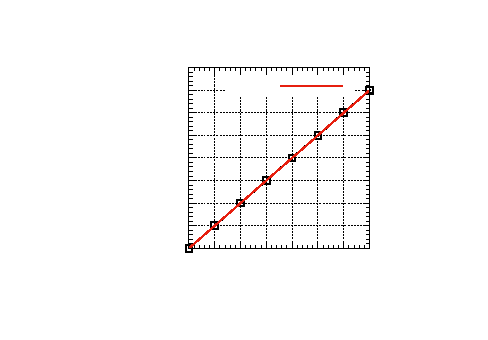
\includegraphics{kinetics/2/2c/mygraph}}%
    \gplfronttext
  \end{picture}%
\endgroup
\\}

% ==========================================================================================
% ==========================================================================================
% ==========================================================================================

\newpage
\section{Equilibrium}

% ==========================================================================================
% ==========================================================================================
% ==========================================================================================

Law of Mass Action (equilibrium constant) for a reaction of form $a\textnormal{A}+b\textnormal{B} \longrightarrow c\textnormal{C}+d\textnormal{D}$:
\begin{equation*}
K_\textnormal{eq} = \frac{[\textnormal{C}]^c[\textnormal{D}]^d}{[\textnormal{A}]^a[\textnormal{B}]^b}
\end{equation*}

van't Hoff Equation
\begin{equation*}
\ln \left(\frac{K_2}{K_1}\right) = \frac{-\Delta H^\circ}{R}\left(\frac{1}{T_2}-\frac{1}{T_1}\right) \textnormal{ or } \ln K_\textnormal{sp} = \frac{-\Delta H^{\circ}}{RT} + \frac{\Delta S^{\circ}}{R}
\end{equation*}

Relationship between equilibrium constants for aqueous systems and for gases:
\begin{equation*}
K_\textnormal{p} = K_\textnormal{c}RT^{\Delta n}
\end{equation*}

Ion product of water:
\begin{equation*}
K_\textnormal{w} = [\textnormal{H$_3$O$^{+}$}][\textnormal{$^{-}$OH}] = \num{1e-14}
\end{equation*}

% ==========================================================================================
% ==========================================================================================
% ==========================================================================================

\subsection{Equilibrium of Acids and Bases}

Definition of pH:
\begin{equation*}
\textnormal{pH} = -\log[\textnormal{H$_3$O$^{+}$}]
\end{equation*}

Definition of pOH:
\begin{equation*}
\textnormal{pOH} = -\log[\textnormal{$^{-}$OH}] = 14-\textnormal{pH}
\end{equation*}

For the reaction HA + H$_2$O $\longrightarrow$ H$_3$O$^{+}$ + A$^{-}$:
\begin{equation*}
\textnormal{\Ka} = \frac{[\textnormal{H$_3$O$^{+}$}][\textnormal{A$^{-}$}]}{[\textnormal{HA}]}
\end{equation*}

For the reaction B + H$_2$O $\longrightarrow$ BH$^{+}$ + $^{-}$OH:
\begin{equation*}
\textnormal{\Kb} = \frac{\textnormal{[BH$^{+}$][$^{-}$OH]}}{\textnormal{[B]}}
\end{equation*}

Relationship between \Ka, \Kb, and \Kw:
\begin{equation*}
\textnormal{\Kw = \Ka \Kb} = \num{1e-14}
\end{equation*}

Definition of \pKa:
\begin{equation*}
\textnormal{\pKa} = -\log(\textnormal{\Ka})
\end{equation*}

Henderson--Hasselbalch equation:
\begin{equation*}
\textnormal{pH = \pKa} + \log \frac{\textnormal{[base]}}{\textnormal{[acid]}}
\end{equation*}

% ==========================================================================================
% ==========================================================================================
% ==========================================================================================

\subsection{Equilibrium and Thermodynamics}

Relationship between standard free-energy change and the equilibrium constant:
\begin{equation*}
\Delta G\not = -RT \ln K
\end{equation*}

Non-standard free energy for a reaction of form $a\textnormal{A}+b\textnormal{B} \longrightarrow c\textnormal{C}+d\textnormal{D}$, where $Q = \frac{[\textnormal{C}]^c[\textnormal{D}]^d}{[\textnormal{A}]^a[\textnormal{B}]^b}$:
\begin{equation*}
\Delta G = \Delta G\not + RT\ln Q
\end{equation*}

% ==========================================================================================
% ==========================================================================================
% ==========================================================================================

\section{Similarity of Equations}

\subsection{Linear Equations with Different Temperatures}

Clausius--Clapeyron Equation:
\begin{equation*}
\ln \frac{P_1}{P_2} = \frac{\Delta H_\textnormal{vap}}{R}\left(\frac{1}{T_2} - \frac{1}{T_1}\right) = \frac{-\Delta H_\textnormal{vap}}{R}\left(\frac{1}{T_1} - \frac{1}{T_2}\right)
\end{equation*}

Arrhenius Equation:
\begin{equation*}
\ln \frac{k_1}{k_2} = \frac{E_\textnormal{a}}{R}\left(\frac{1}{T_2} - \frac{1}{T_1}\right) = \frac{-E_\textnormal{a}}{R}\left(\frac{1}{T_1}-\frac{1}{T_2}\right)
\end{equation*}

van't Hoff Equation:
\begin{equation*}
\ln \frac{K_1}{K_2} = \frac{\Delta H^\circ}{R}\left(\frac{1}{T_2}-\frac{1}{T_1}\right) = \frac{-\Delta H^\circ}{R}\left(\frac{1}{T_1}-\frac{1}{T_2}\right)
\end{equation*}

van't Hoff Equation with \Ksp\ and entropy, plot $\ln K_\textnormal{sp}$ vs. $1/T$:
\begin{equation*}
\Delta H^{\circ} - T\Delta S^{\circ} = \Delta G^{\circ} = -RT \ln K_\textnormal{sp}
\end{equation*}
\begin{equation*}
\ln K_\textnormal{sp} = \frac{-\Delta H^{\circ}}{RT} + \frac{\Delta S^{\circ}}{R}
\end{equation*}

\subsection{Summations}

Standard entropy of reaction, where $n$ and $m$ are coefficients in the balanced reaction equation:
\begin{equation*}
\Delta S\not_\textnormal{rxn} = \sum{n\Delta S\not(\textnormal{products})}-\sum{m\Delta S\not(\textnormal{reactants})}
\end{equation*}

Standard enthalpy of reaction, where $n$ and $m$ are coefficients in the balanced reaction equation:
\begin{equation*}
\Delta H\not_\textnormal{rxn} = \sum{n\Delta H\not_\textnormal{f}(\textnormal{products})}-\sum{m\Delta H\not_\textnormal{f}(\textnormal{reactants})}
\end{equation*}

Standard free energy of reaction, where $n$ and $m$ are coefficients in the balanced reaction equation:
\begin{equation*}
\Delta G\not_\textnormal{rxn} = \sum{n\Delta G\not_\textnormal{f}(\textnormal{products})}-\sum{m\Delta G\not_\textnormal{f}(\textnormal{reactants})}
\end{equation*}

% ==========================================================================================
% ==========================================================================================
% ==========================================================================================


% ==========================================================================================
% ==========================================================================================
% ==========================================================================================

\section{Other}

Relationship between mass defect and energy released: 
\begin{equation*}
\Delta E = (\Delta m)c^2
\end{equation*}


























\end{document}

% ==========================================================================================
% ==========================================================================================
% ==========================================================================================
